\documentclass{handout}

\SetInstructor{Lt Col James Phillips}
\SetCourseTitle{ECE231: Electrical Circuits and Systems I}
\SetSemester{Spring 2016}
\SetHandoutTitle{Lecture 7: Mesh Current Analysis}
%\SetDueDate{1 Jan 2016}
%\ShowAllBlanks

\showsoln \setsolncolor{red}

\begin{document}
\maketitle

\textbf{Upcoming events}
\begin{enumerate}
\item HW \#3 due Lesson 10
\item Problem set \#2 due Lesson 10
\item Quiz \#2 during Lesson 10
\end{enumerate}

\textbf{OBJECTIVES:}
\begin{enumerate}
\item Demonstrate the ability to write mesh current equations for a given circuit
\item Demonstrate the ability to solve for unknown circuit parameters using mesh current analysis
\end{enumerate}

\textbf{READING}
\begin{description}
\item [Required]:
\begin{itemize}
\item  Textbook, sections 3.2, pages 92--100
\end{itemize}
\item [Optional]: None
\end{description}

\textbf{HOMEWORK}
\begin{description}
\item [Required textbook problems]: 3.14, 3.18, 3.22 --- Due Lesson 8
\item [Recommended textbook problems]: 3.13
\item[Other]: Lab \#2 --- Due Lesson 9
\end{description}


\section{What is Mesh Current Analysis?}
Similar to Node Voltage Analysis, it is a more efficient method for solving circuits than being forced to rely on element and connection constraints.  What we write instead are equations for {\em Mesh Currents}.  To do this we have to first answer the question, what is a mesh?

\soln{1in}{
A mesh is a loop that does not contain any other loops inside of it
}

In Figure \ref{fig: SimpleLoopCounting}, loops 1 \& 2 are meshes, but loop 3 is not.

\begin{figure} [h t b]
\centering
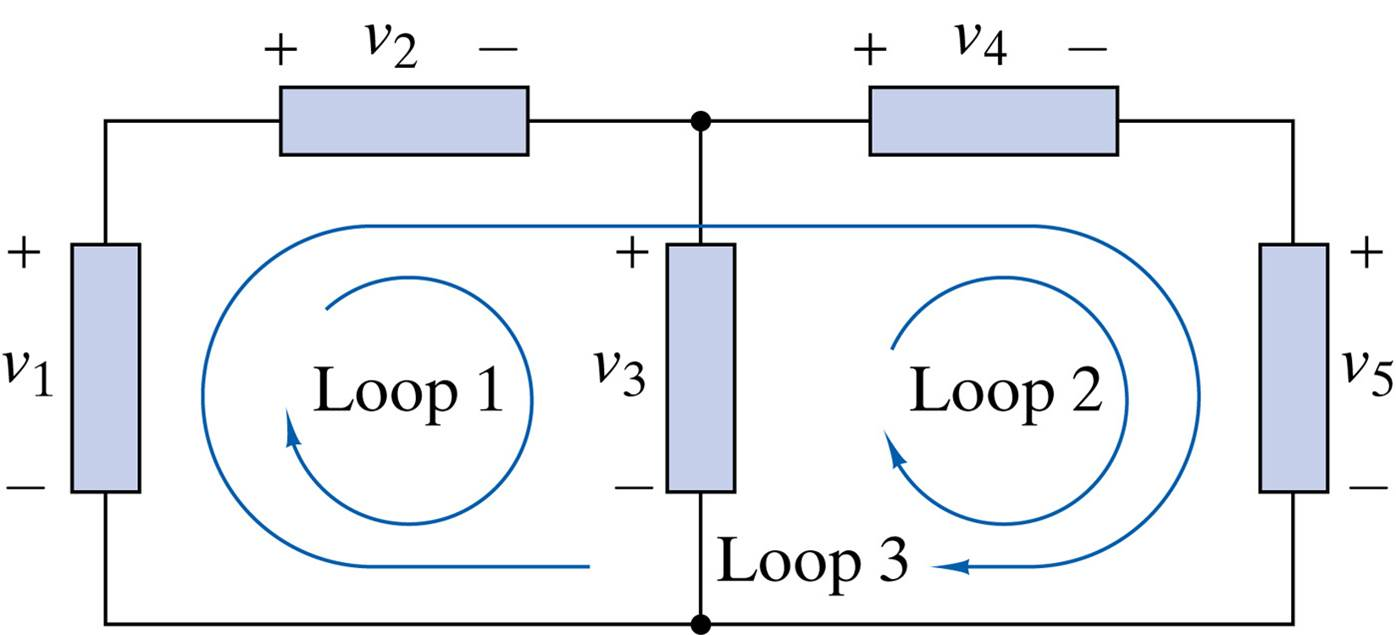
\includegraphics[width=0.4\textwidth]{SimpleLoopCounting.jpg}
\caption{Loops 1 \& 2 are meshes; loop 3 is not}
\label{fig: SimpleLoopCounting}
\end{figure}

\newpage
\clearpage
\pagebreak

\section{Circuits with NO CURRENT sources}
This section will give steps for wrining Mesh Current eqautions and then will give examples.  The steps will likely not make much sense until we look at a couple of examples.

\subsection{Steps for writing Mesh Current Equations}
\soln{4in}{
\begin{enumerate}
\item Assign a current to each mesh
\item Assign a voltage (magnitude and polarity) to each device in the circuit
\item Write Kirchhoff's Voltage Law (KVL) equations for each mesh
\item Use device $i$--$v$ characateristics to rewrite KVL eqations from the previous step
\item Rewrite equations in standard (matrix) form
\end{enumerate}
}

\subsection{Examples}
\textbf{Example 1:} In the circuit shown in Figure \ref{fig: MeshAnalysisEx1}, use mesh current analysis to find the voltage drop across the $25\ k\Omega$ resistor and the current out of the (positive terminal) source.  

\begin{figure} [h t b]
\centering
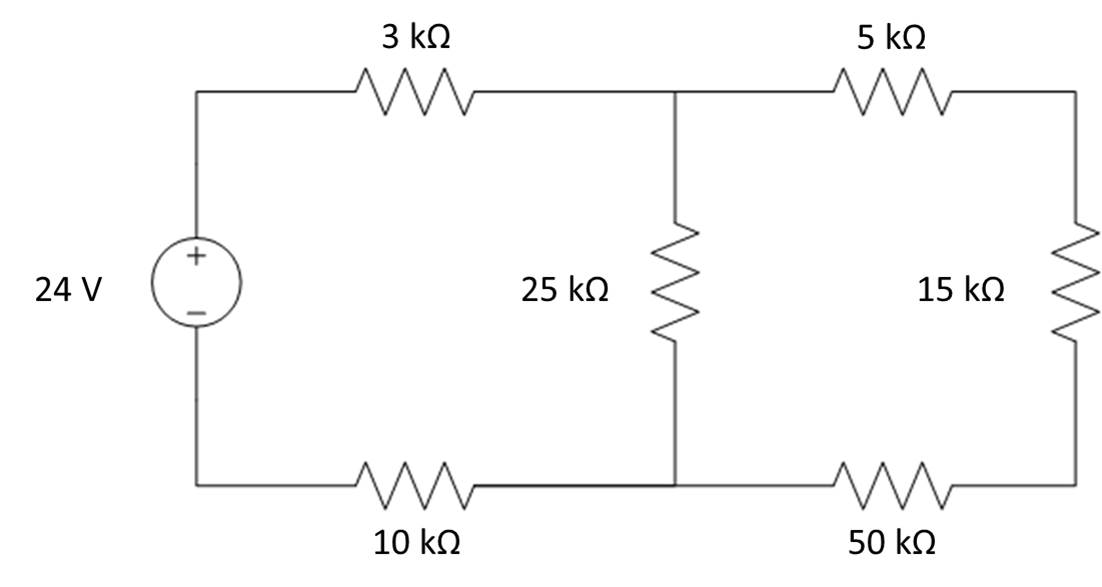
\includegraphics[width=0.4\textwidth]{MeshAnalysisEx1.jpg}
\caption{Circuit to accompany example 1}
\label{fig: MeshAnalysisEx1}
\end{figure}

\soln{6in}{
\begin{figure} [h t b]
\centering
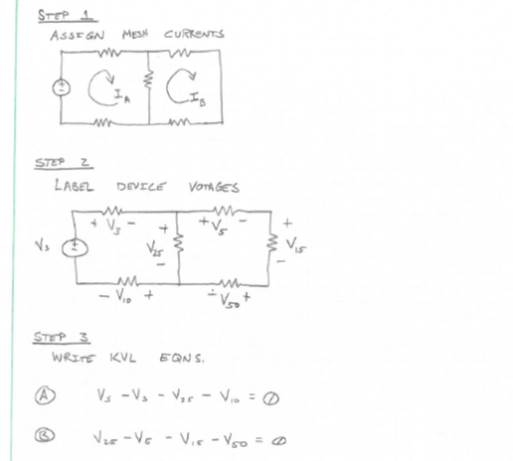
\includegraphics[width=0.5\textwidth]{MeshAnalysisEx1solnA.jpg}
\end{figure}

\begin{figure} [h t b]
\centering
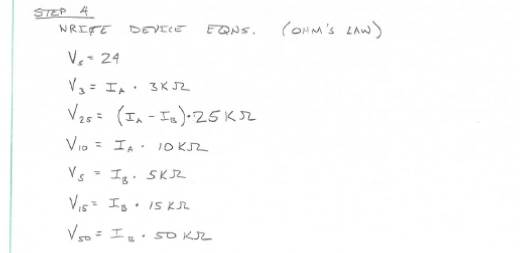
\includegraphics[width=0.7\textwidth]{MeshAnalysisEx1solnB.jpg}
\end{figure}

\begin{figure} [h t b]
\centering
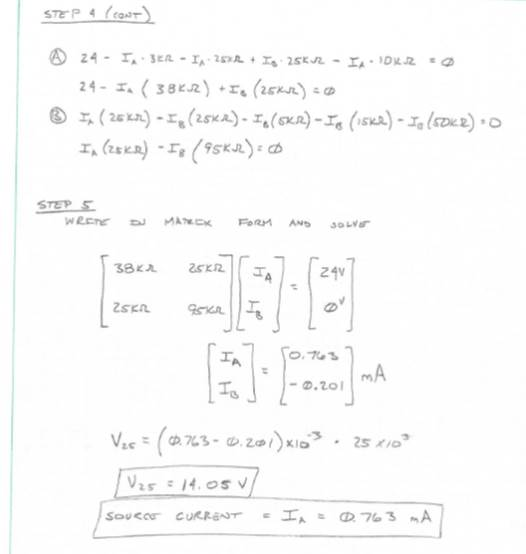
\includegraphics[width=0.7\textwidth]{MeshAnalysisEx1solnC.jpg}
\end{figure}
}

\newpage
\clearpage
\pagebreak

\textbf{Example 2:} Let's rework the same example, just add a third mesh.  See Figure \ref{fig: MeshAnalysisEx2}

\begin{figure} [h t b]
\centering
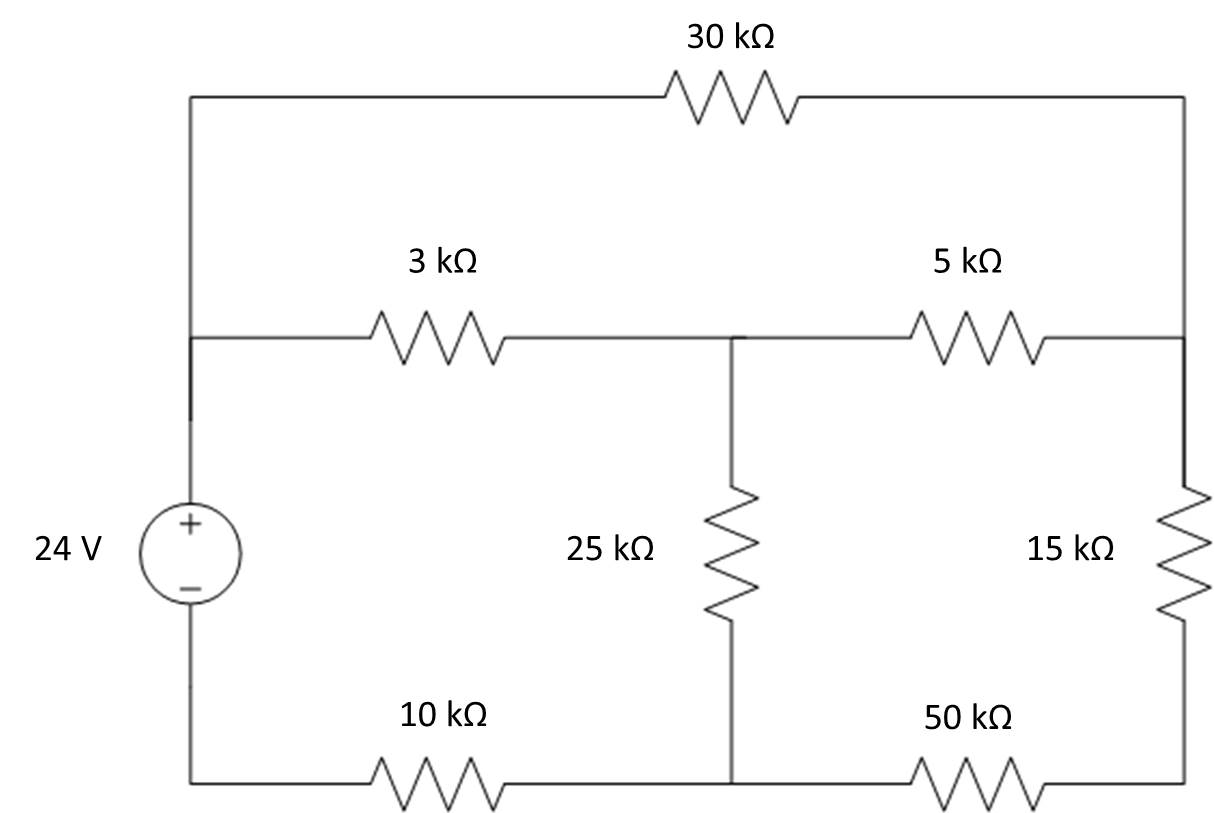
\includegraphics[width=0.4\textwidth]{MeshAnalysisEx2.jpg}
\caption{Circuit to accompany example 2}
\label{fig: MeshAnalysisEx2}
\end{figure}

\soln{6in}{
\begin{figure} [h t b]
\centering
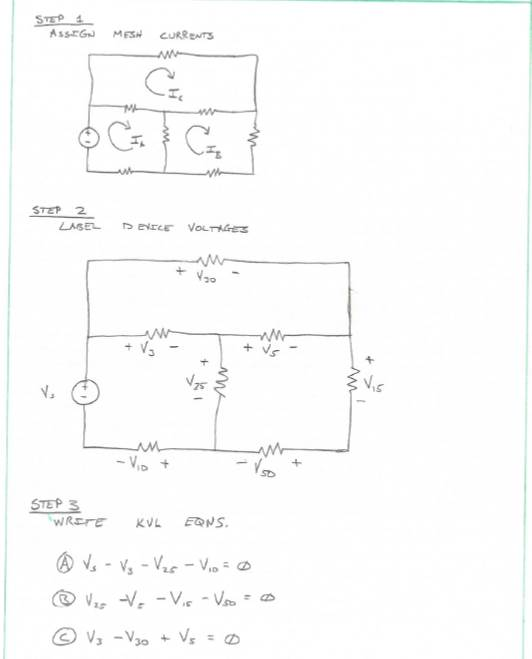
\includegraphics[width=0.55\textwidth]{MeshAnalysisEx2solnA.jpg}
\end{figure}

\begin{figure} [h t b]
\centering
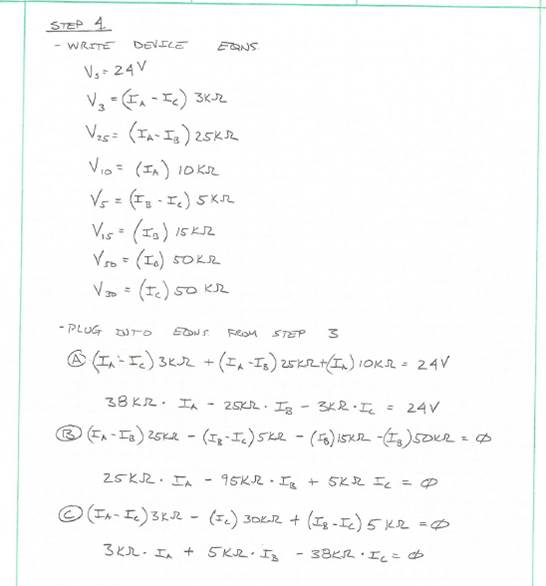
\includegraphics[width=0.7\textwidth]{MeshAnalysisEx2solnB.jpg}
\end{figure}

\begin{figure} [h t b]
\centering
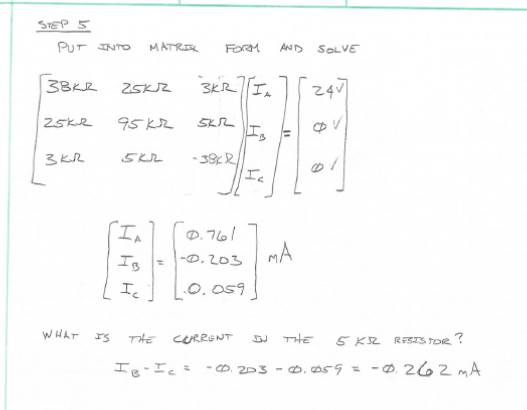
\includegraphics[width=0.7\textwidth]{MeshAnalysisEx2solnC.jpg}
\end{figure}
}

\newpage
\clearpage
\pagebreak

\section{Mesh Analysis for circuits with current sources}
Recall from last lesson, when we used nodal analysis on circuits with voltage sources, the set up of the problem was a little more challenging, however, the actual solution was simplified.  This will same idea applies to using Mesh Analysis on circuits with current sources.

Like las lesson we will introduce 3 techniques for solving these types of circuits.

\subsection{Method 1: Source Transformation}
If the current source is in parallel with a resistor, we can convert it to an equivalent voltage source.  If we eliminate all current sources using this method, we can revert back to the process shown above. 

\textbf{Example 3:} Use Mesh Analysis to find the current through the $3\ k\Omega$ resistor in Figure \ref{fig: MeshAnalysisEx3}
\begin{figure} [h t b]
\centering
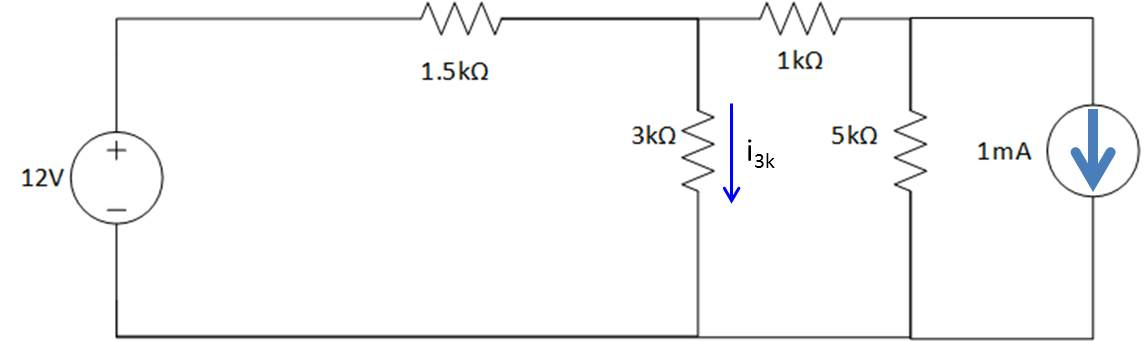
\includegraphics[width=0.6\textwidth]{Example3.jpg}
\caption{Circuit to accompany example 3}
\label{fig: MeshAnalysisEx3}
\end{figure}

\soln{6in}{
\begin{figure} [h t b]
\centering
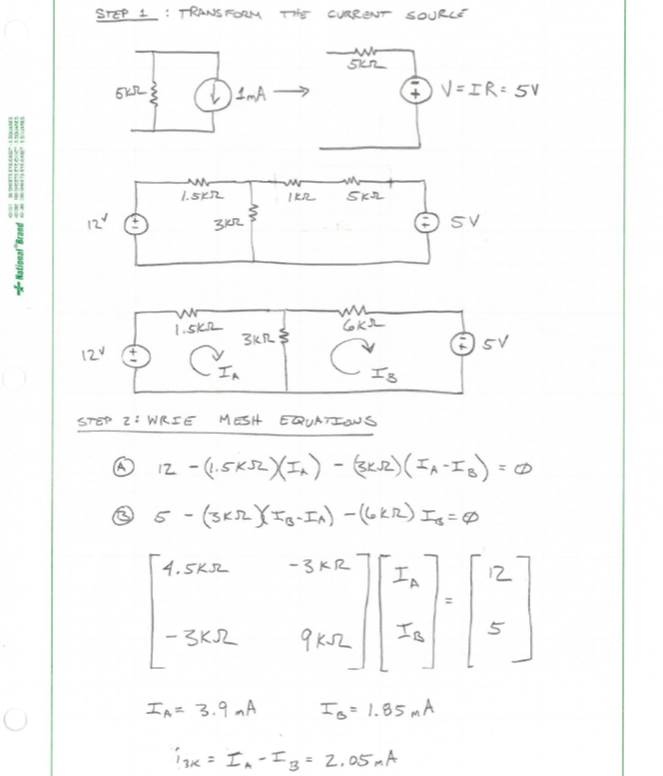
\includegraphics[width=0.55\textwidth]{Example3soln.jpg}
\end{figure}
}

\newpage
\clearpage
\pagebreak

\subsection{Method 2: Source is part of only 1 mesh}
This method is really the simplest of all.  If the source is only part of one mesh, we know the mesh current for that mesh; namely the value of the current source. 

\textbf{Example 4:} Redo example 3 using method 2.
\soln{6in}{
\begin{figure} [h t b]
\centering
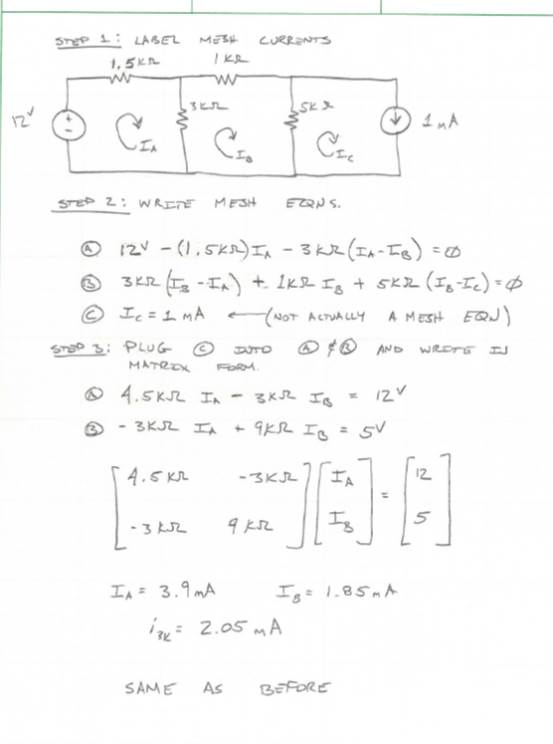
\includegraphics[width=0.7\textwidth]{Example4soln.jpg}
\end{figure}
}

\newpage
\clearpage
\pagebreak

\subsection{Method 3: Supermeshes}
If a current source is shared by 2 meshes, we can combine them into a {\em Supermesh}.  To do this, we identify mesh currents just as we would have before, but we do not write mesh equations for the meshes that share the current source; rather, we just write one supermesh equation.  We do not write any mesh equations that include the current source or any other elements that share the branch with the current source.  Our last equation simply relates the mesh currents to the current source.  Like the other methods, this is best illustrated by an example

\textbf{Example 5:} Find the voltage drop across the $1\ k\Omega$ resistor in Figure \ref{fig: MeshAnalysisEx5}. Use Mesh Analysis method 3
\begin{figure} [h t b]
\centering
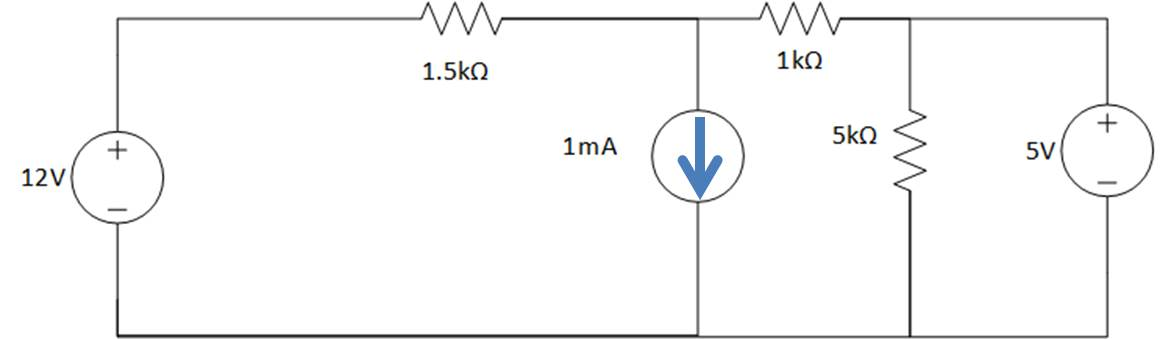
\includegraphics[width=0.6\textwidth]{Example5.jpg}
\caption{Circuit to accompany example 5}
\label{fig: MeshAnalysisEx5}
\end{figure}

\soln{6in}{
\begin{figure} [h t b]
\centering
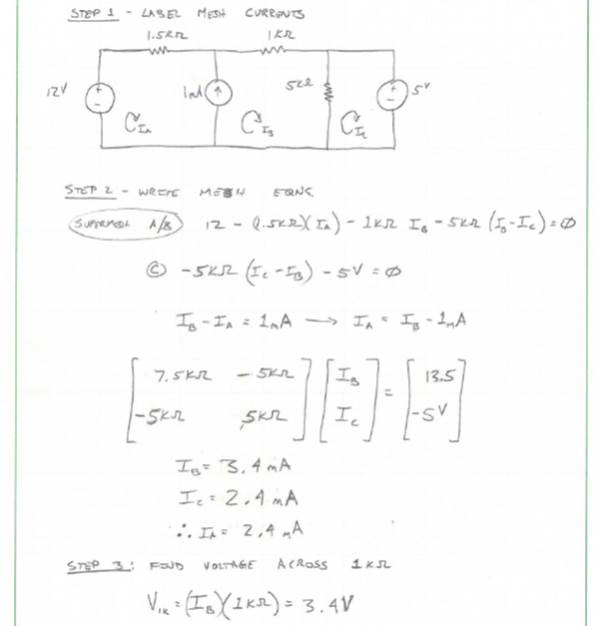
\includegraphics[width=0.7\textwidth]{Example5soln.jpg}
\end{figure}
}

\newpage
\clearpage
\pagebreak

\textbf{Example 6:} Use mesh analysis to find the voltage across the $1A$ source in the circuit shown in Figure \ref{fig: MeshAnalysisEx6}
\begin{figure} [h t b]
\centering
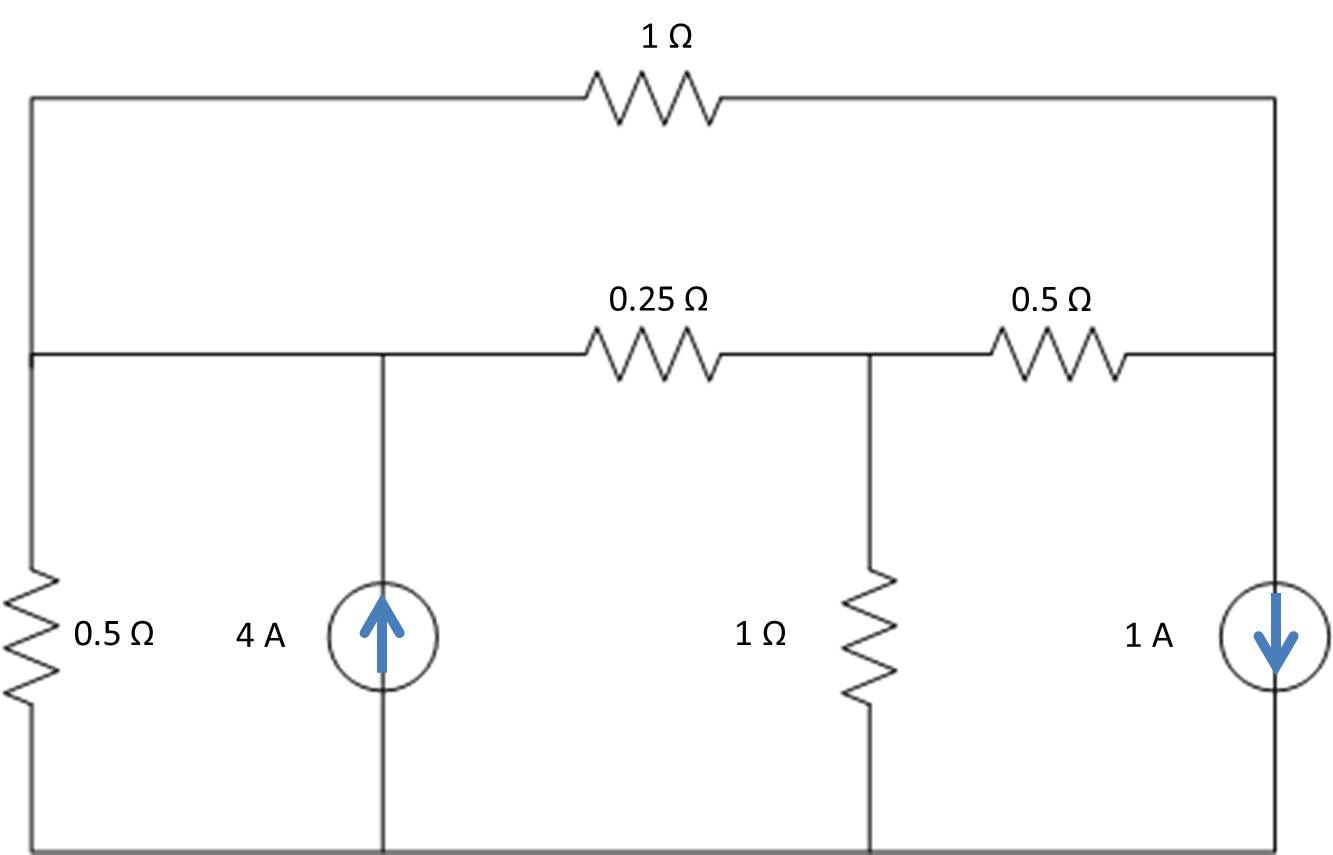
\includegraphics[width=0.4\textwidth]{Example6.jpg}
\caption{Circuit to accompany example 6}
\label{fig: MeshAnalysisEx6}
\end{figure}

\soln{6in}{
\begin{figure} [h t b]
\centering
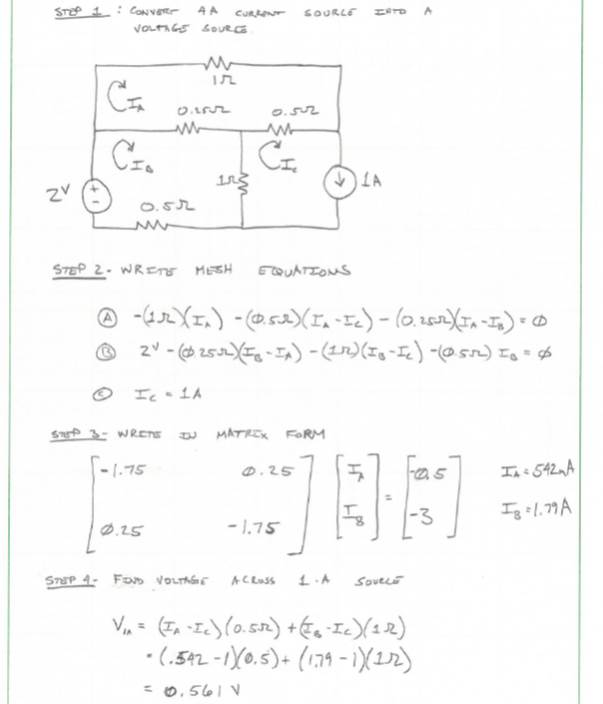
\includegraphics[width=0.6\textwidth]{Example6soln.jpg}
\end{figure}
Notice that this matches our results we got using nodal analysis in lesson 6
}

\newpage
\clearpage
\pagebreak






\end{document}


% Equation Array Example Code
%\begin
%{eqnarray}
%P_R &=& i_R^2R \nonumber \\
%P_R &=& (100\ mA)^2 \times 100\ \Omega \nonumber \\
%P_R &=& (100 \times 10^{-3}\ A)^2 \times 100\ \Omega \\
%P_R &=& 10000 \times 10^{-6}\ A^2  \times 100\ \Omega \nonumber \\
%P_R &=& 1\ W  \nonumber
%\end{eqnarray} 

% Figure Example Code
%\begin{figure} [h t b]
%\centering
%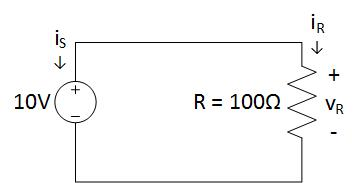
\includegraphics[width=0.5\textwidth]{OhmsLawExampleSolution.jpg}
%\caption{Ohm's Law example circuit}
%\label{fig: OhmsLawExampleSolution}
%\end{figure}

%Table Example Code
%\begin{table}[h]
%\centering
%\begin{tabular}{|l|c|c|}
%\hline
%Prefix & Abbreviation & Value \\
%\hline \hline
%Giga & $G$ & $10^9$ \\
%Mega & $M$ & $10^6$ \\
%Kilo & $k$ & $10^3$ \\
%\hline
%milli & $m$ & $10^{-3}$ \\
%micro & $\mu$ & $10^{-6}$ \\
%nano & $n$ & $10^{-9}$ \\
%pico & $p$ & $10^{-12}$ \\
%\hline
%\end{tabular}
%\caption{Engineering prefixes and values}
%\label{tab: Eng Prefixes}
%\end{table}
